\section{Motivation}

    In this section we first motivate online iterative compilation by showing the deleterious effects of choosing the wrong inputs for the
    offline case. Then we go on to show the unsuitability of previously proposed program version comparison metrics.

    \begin{figure}[t!]
        \centering
        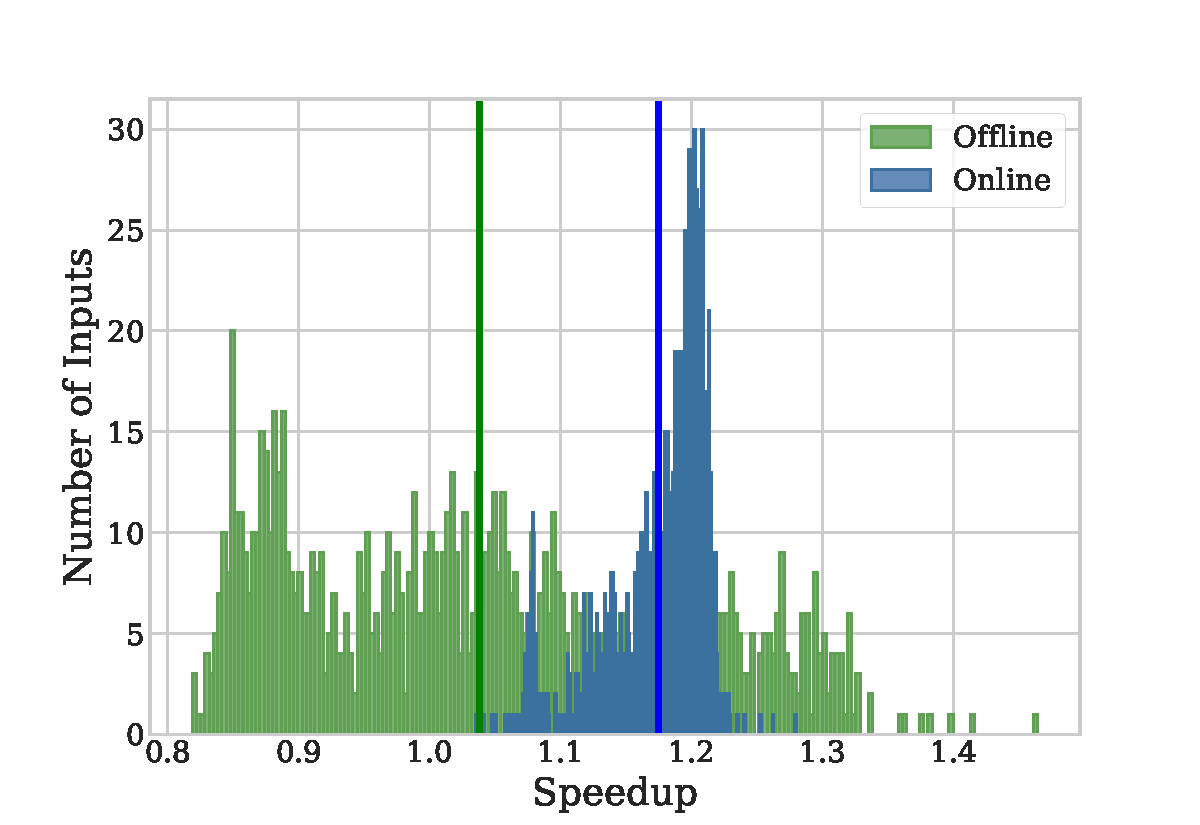
\includegraphics[width=0.5\textwidth]{figs/motivation-online.pdf}
        \caption{
            Histograms of speedup over \texttt{-O3} for each of the 1,000 inputs of \texttt{susan\_c}. The green histogram shows the
            speedup when using the optimization sequence selected by offline \itercomp, the blue one is the speedup using the optimization
            sequence selected by an online-like approach. \FIXME{Beware Daltonism!}
        }
        \label{fig:motivation-online}
    \end{figure}

    We performed offline iterative compilation on \texttt{susan\_c} to find the optimization settings that maximize the average performance
    over \FIXME{five} randomly chosen inputs from a set of \FIXME{1,000} provided by \textit{KDataSets} benchmark
    suite~\cite{chen10,chen12a}. The green histogram in Figure~\ref{fig:motivation-online} shows the speedups for all \FIXME{1,000} inputs
    of that chosen optimization setting versus \texttt{-O3}. The dark green line shows the average speedup for all those inputs. The
    \FIXME{five} training inputs are all in the top \FIXME{twelve} performing inputs. On the other hand, the chosen optimization does
    poorly on other inputs, often causing a slowdown and yielding only a slight speedup of 6\% on average.
    
    The blue bars in Figure~\ref{fig:motivation-online} show a different approach. Here the iterative compilation proceeds by evaluating
    each optimization on \FIXME{five} inputs. Each input is evaluated only once during the search, but the search is provided with oracle
    knowledge about the unoptimized runtime for the inputs, giving a perfect work metric. The environment of the search constantly changes
    in the same way as for online iterative compilation. The best optimization for this case never degrades performance compared to
    \texttt{-O3} and is on average 13\% better than the offline approach. The online case, considering truly representative inputs, leads
    to superior performance, if a suitable work metric can be found that comes close to the oracle.

    \begin{figure}[t]
        \centering
        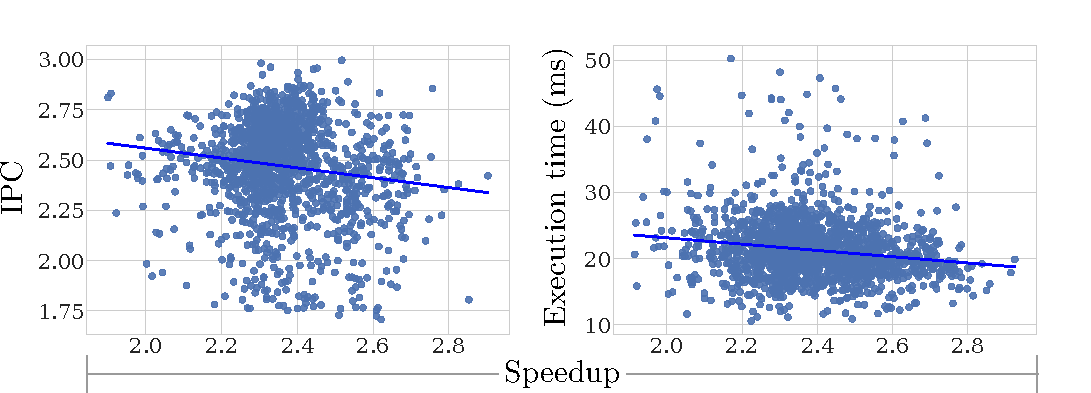
\includegraphics[width=0.5\textwidth]{figs/motivation-metric.pdf}
        \caption{
            Relationship between IPC and execution time vs optimization speedup for 500 different binaries of \texttt{susan\_c}.
            Each point represents averages over all inputs.
        }
        \label{fig:motivation-metric}
    \end{figure}
    
    Prior to this paper there were two proposed metrics to correlate with program efficiency. The first is simply to use runtime, ignoring
    the work aspect. This functions well when the inputs all require similar effort. When that is not the case it bears little or no
    correlation to efficiency. The second approach is \textit{instructions per cycle}~(IPC), suggested by~\citep{fursin07}. While IPC seems
    promising in the sense that faster instruction execution is a good thing, this is belied by the simple observation that adding
    redundant NOPs to a program will increase IPC while also slowing the program down. Figure~\ref{fig:motivation-metric} shows the
    relationship between execution time, IPC and speedup for different optimizations of \texttt{susan\_c}, averaged across all inputs.
    Neither IPC nor execution time correlate well, and so neither can be used for iterative compilation. We need a work efficiency metric
    which can approximate speedup instead, using only a single execution. \FIXME{HJL: exec time avg over all inputs, why not good?}

    In the remainder of this paper we present our work efficiency metric and demonstrate its utility for iterative compilation.
    
%<<<<<<< Updated upstream
%The success of \itercomp relies on having representative inputs for the target program to be optimized. If the developers cannot predict
%what will be the typical usage of the application or that typical usage changes over time, then \itercomp might fail making the application
%faster for the user.
%
%\begin{figure}[t!]
%    \centering
%    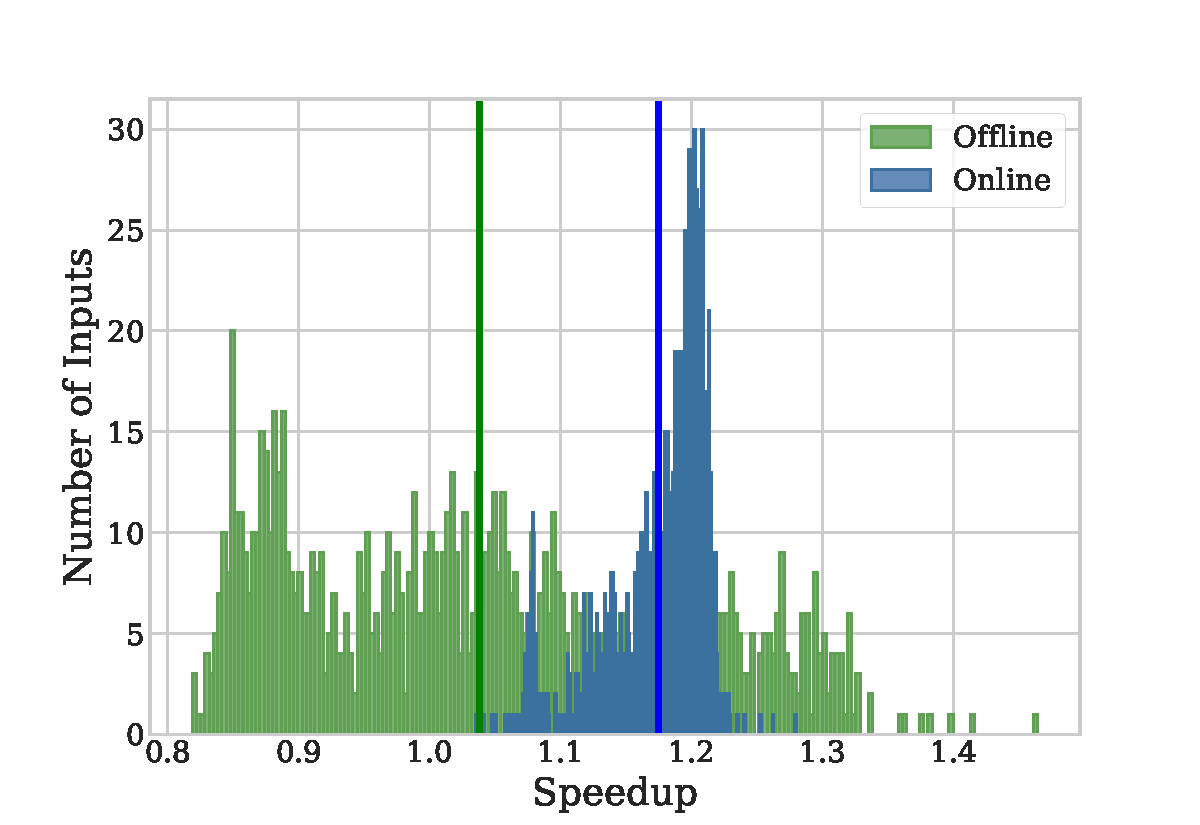
\includegraphics[width=0.5\textwidth]{figs/motivation-online.pdf}
%    \caption{Histograms of speedup over \texttt{-O3} for each of the 1,000 inputs of \texttt{susan\_c}. The green histogram shows the speedup when using
%    the optimization sequence selected by offline \itercomp, the blue one is the speedup using the optimization sequence selected by an
%    online-like approach.}
%    \label{fig:motivation-online}
%\end{figure}
%
%To show this, we performed offline \itercomp on \texttt{susan\_c} from the \textit{KDataSets} benchmark suit~\cite{chen10,chen12a} using a
%small subset of its inputs to identify the best-performing optimization sequence. In Figure~\ref{fig:motivation-online}, the green bars are
%the histogram of speedups compared to \red{LLVM?} \texttt{-O3} for each individual input, while the dark green line shows the speedup
%averaged over all inputs. Despite the selected optimization sequence being the best for some inputs, we see that it delivers, on average,
%6\% of performance improvement, but gives slows down performance for nearly of the inputs. This example shows that randomly choosing an
%input set to use for offline \itercomp can be counterproductive.
%
%The blue bars \red{zw: the reviewer won't be able to see the difference if the paper is printed in black and white.} in
%Figure~\ref{fig:motivation-online} show a different approach where during \itercomp the speedup of each optimization sequence is again
%measured on a small input subset but this subset changes for every optimization sequence. This is similar to how online \itercomp would
%have to work, using each input only once. This might introduce errors, since the speedups we measure for each optimization sequence are not
%strictly comparable, they are measured on different workloads. But in the end the histogram shows that being able to test more inputs
%allows us to make better informed decisions. The optimization sequence we selected never degrades performance compared to \texttt{-O3} and
%is on average 13\% better than the offline approach.
%
%\begin{figure}[t]
%    \centering
%    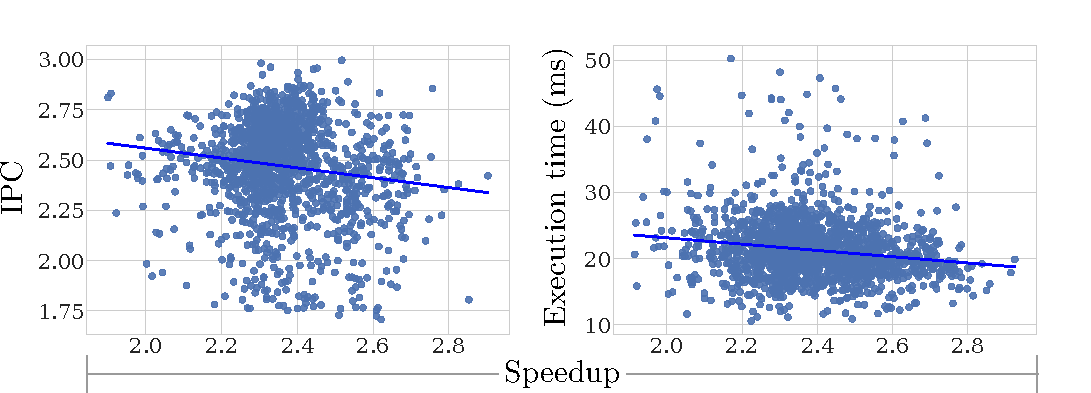
\includegraphics[width=0.5\textwidth]{figs/motivation-metric.pdf}
%    \caption{Relationship between IPC and execution time vs optimization speedup for 500 different binaries of \texttt{susan\_c}. The binaries are compiled using different optimization sequences. Each point represents
%	averages over a distinct subsets of its inputs.}
%    \red{ZW: Perhaps take out the blue line (execution time). It is rather confusing. }
%    \label{fig:motivation-metric}
%\end{figure}
%
%This is not an entirely surprising result. Evaluating our optimization decisions on more inputs decreases the chances of optimizing for an
%unrepresentative input. Despite that offline \itercomp is still the preferred way. Measuring the speedup caused by an optimization requires
%running the same input \textit{at least twice}, one of the optimized and one for the baseline binary. This is either infeasible or
%undesirable in a realistic online \itercomp scenario. There are two existing workarounds to this problem: directly comparing the
%\textit{execution time} of each run against previous runs or directly comparing the \textit{instructions per cycle}~(IPC)~\citep{fursin07}.
%Neither metric is a good proxy for speedup. Figure~\ref{fig:motivation-metric} plots the measured IPC and execution time versus the real
%speedup for 500 different binaries of the \texttt{susan\_c} benchmark. IPC, execution time, and speedup are averaged over distinct subsets of its inputs.
%Both metrics have no direct correlation with speedup. Different inputs require a different amount of work which dominates the changes in execution time. IPC on
%the other hand might improve with a more efficient binary but the opposite can also be true. For example,
%replacing many one-cycle instructions by fewer multi-cycle instructions.
%%inserting \texttt{NOP} statements will usually improve IPC.
%
%In the remaining of this paper, we describe our work efficiency metric, which provides a new way for approximating optimization speedup
%through a single run. We show that by utilizing this metric, a highly effective online \itercomp methodology can be built.
